% Chapter Template

\chapter{Implementação de modelo ML} % Main chapter title

\label{ChapterX} % Change X to a consecutive number; for referencing this chapter elsewhere, use \ref{ChapterX}

%----------------------------------------------------------------------------------------
%	SECTION 1
%----------------------------------------------------------------------------------------

\section{Considerações Iniciais}

Conforme Vincent, o foco deve estar em entender com profundidade o problema, dar um passo atrás e ser humilde, se para você, o problema ainda não está claro. Não se deve focar, em primeiro lugar na solução, e pensar o problema como algo meramente analítico ("Vou ajustar uma rede neural e encontrar os melhores hiperparâmetros e o problema será resolvido!). De modo geral, o que mas importa é todo o conjunto de componentes ao redor do modelo de ML, não o modelo em si. As componentes seriam:

\begin{itemize}
\item Quais dados temos acesso?
\item Qual é a utilidade do modelo para o usuário final?
\item Como seria feito o monitoramento do modelo? Quão complicado seria corrigir erros podem surgir em produção? Corrigir erros de uma regressão linear é muito mais fácil e rápido que corrigir os erros de uma rede neural com milhares/milhões de parâmetros
\item Um sistema simples de regras poderia desempenhar tão bem quanto um modelo de ML?
\item Como avaliar a qualidade do modelo proposto? Há algum benchmark? Pode-se criar um benchmark?
\item Fazer um desenho à mão de toda a arquitetura é uma boa ideia
\end{itemize}

%-----------------------------------
%	SUBSECTION 1
%-----------------------------------
\section{Particionamento dos Dados}
\begin{figure}[H]
\centering
\caption{Data Partitioning}
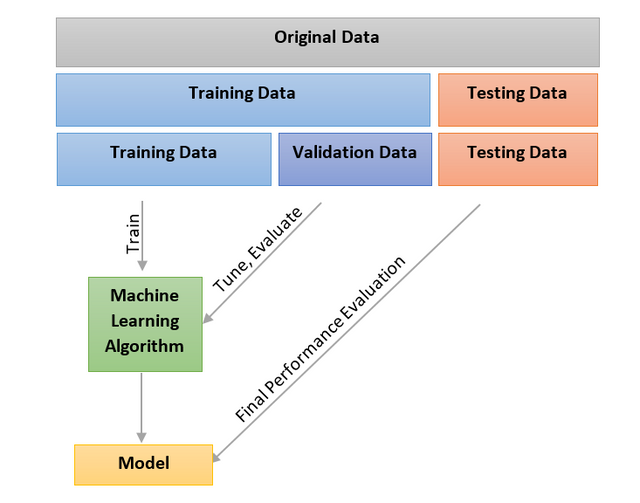
\includegraphics[scale=1.0]{validation.png}
\end{figure}

\begin{itemize}
\item We usually devide the data to train and test set. We will not touch test set until the end of the computation and the final perpormance evaluation. Then, we can devide the train set to train and validation sets. We use the validation data set to tune the model.
\item Traditional train test method suffer from high variance test problem. It means tha by changing the test set the result of the prediction changes. To over come this problem we use k-fold validation method in our train and validation set

\item Separating samples into training and test sets is not always enough. There can be various reasons for duplicate samples that appear in both sets, and it is important to detect and remove these duplicates. For example, one of the most used datasets in Computer Vision, CIFAR, is shown to contain duplicate samples in training and test sets. This becomes more of a problem for models that are trained on huge amounts of data such as BERT and GPT-3. Best practices: Remove duplicates before splitting the data, check for partial duplicates as well, sort by different columns, and examine the data.

\end{itemize}    

%-----------------------------------
%	SUBSECTION 2
%-----------------------------------

\section{Passo a Passo}

\begin{enumerate}
\item Estudo profundo das fontes de informação disponíveis (banco de dados, API's, planilhas);

\item Identificação de variáveis relevantes. Essa etapa costuma assumir um dos dois caminhos seguintes:
\begin{enumerate}
    \item Um seleção de variáveis é feita, com base no conhecimento do negócio envolvido. Se o cientista de dados não conhece bem o campo de conhecimento envolvido, fica difícil fazer isso. Então, consultar especialistas é extremamente recomendado
    
    \item Milhões, milhares de variáveis são escolhidas e jogadas para treinar o modelo mais para frente.
\end{enumerate}

\item Fazer Exploratory Data Analysis do conjunto de dados:

\begin{itemize}
    \item Há dados faltantes?
    \item Há dados que não fazem sentido algum? Por exemplo, uma pessoa tem altura negativa!
    \item As strings, para uma determinada coluna, são consistentes? Por exemplo, a string que se refere a cidade "New York" possui diferentes formatos, e.g., "NEWYORK", "ny", "NY", "new york".
    
\end{itemize}

\section{Considerações sobre predição}
Um modelo de aprendizado de máquina supervisionado treinado com um conjunto de dados de treino é capaz de fazer predições e, por meio dele, conseguimos testar sua performance no conjunto de dados de teste.

Contudo, é de extrema importância que um modelo de ML, em produção, em uma empresa ou aplicação na vida real passe por uma análise de sua performance com um conjunto de dados que só será obtido no futuro. 

Um modelo que classifica se uma reserva de hotel será cancelada, com o snapshot dos dados atuais "apenas" classifica as observações em não canceladas ou canceladas. Entretanto, a gerência do hotel (usuário do modelo) está interessada especificamente em prever, no futuro, um cancelamento. Classificar uma observação atual em não cancelada ou cancelada é algo distinto de prever, no futuro, um cancelamento de reserva de hotel.

Sendo assim, é necessário que de tempos em tempos, com novas safras de dados e as previsões feitas antecipadamente sejam estudadas. É necessário simular o uso final do modelo! 

\end{enumerate}